% Name: Secant and tangent lines
% Description: The secant through P and Q, and the tangent at P that it approaches as Q moves toward P.
% Tags: derivative, tangent, secant, slope

\usetikzlibrary{arrows.meta}

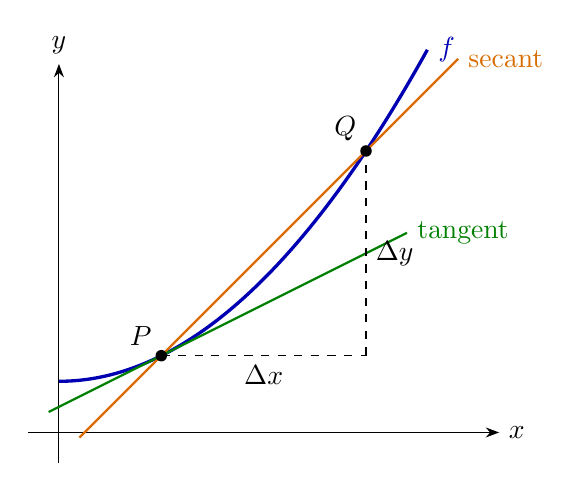
\begin{tikzpicture}[>={Stealth}, scale=1.3]
  \draw[->] (-0.3,0) -- (4.3,0) node[right] {$x$};
  \draw[->] (0,-0.3) -- (0,3.6) node[above] {$y$};
  \draw[very thick, blue!70!black, domain=0:3.6, samples=60, smooth]
    plot (\x, {0.25*\x*\x + 0.5}) node[right] {$f$};
  \draw[thick, orange!85!black, domain=0.2:3.9] plot (\x, {\x - 0.25}) node[right] {secant};
  \draw[thick, green!50!black, domain=-0.1:3.4] plot (\x, {0.5*\x + 0.25}) node[right] {tangent};
  \draw[dashed] (1,0.75) -- (3,0.75) node[midway, below] {$\Delta x$};
  \draw[dashed] (3,0.75) -- (3,2.75) node[midway, right] {$\Delta y$};
  \fill (1,0.75) circle (1.6pt) node[above left] {$P$};
  \fill (3,2.75) circle (1.6pt) node[above left] {$Q$};
\end{tikzpicture}
